\section*{Условие}
Используя хвостовую рекурсию, разработать эффективную программу, позволяющую найти:
\begin{enumerate}
	\item Длину списка (по верхнему уровню);
 	\item Сумму элементов;
  \item Сумму элементов числового списка, стоящих на нечетных позициях исходного списка (нумерация с 0).
\end{enumerate}
Для каждой программы реализовать два варианта: с использованием отсечения и без использования отсечения.  

Убедиться в правильности результатов.

\textbf{Для одного} из вариантов \textbf{ВОПРОСА} и одного из заданий \textbf{составить
таблицу}, отражающую конкретный порядок работы системы:

Т.к. резольвента хранится в виде стека, то состояние резольвенты требуется отображать
в столбик: (вершина – сверху). Новый шаг надо начинать с нового состояния резольвенты.  

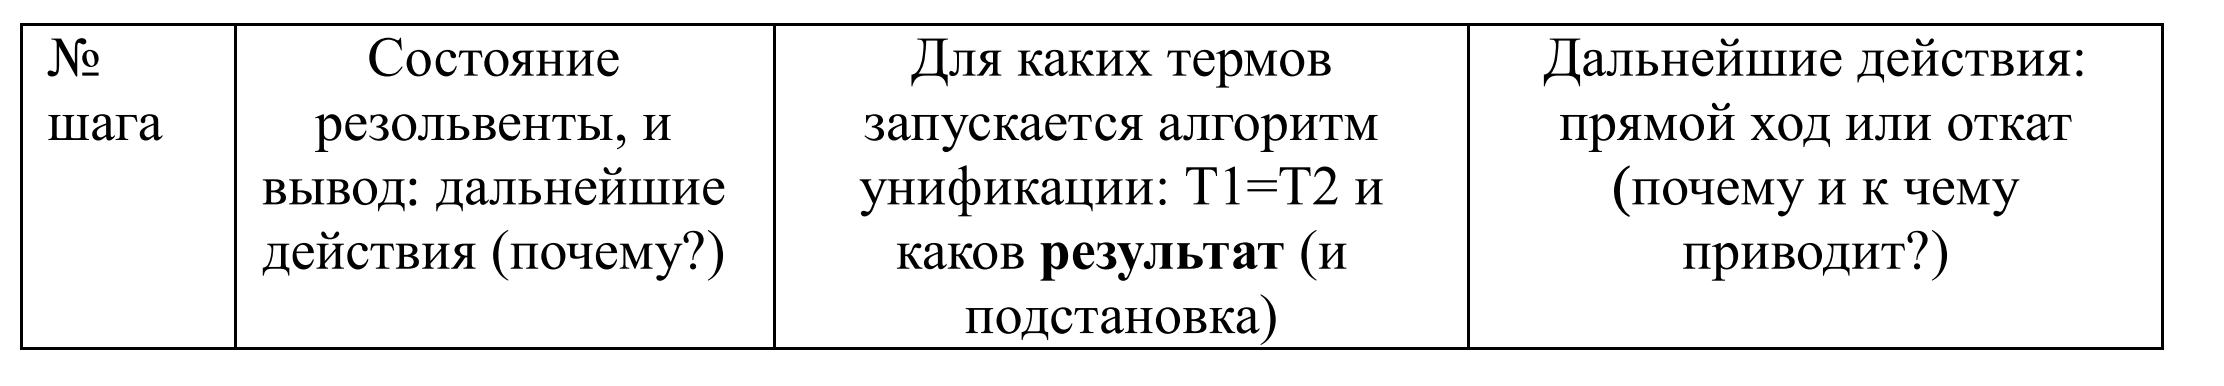
\includegraphics[scale=0.4]{./inc/img/tb_tmpl}

\section*{Решение}
\lstinputlisting[caption={Решение}, label={lst:t1}, language=Prolog]{../src/main.pro}

В Таблице \ref{tbl:1} представлен порядок поиска ответа на вопрос 1.

\begin{landscape}
  \setlength{\LTcapwidth}{\linewidth}
  \begin{longtable}{|c|c|c|c|c|}
      \caption[Порядок формирования результата для 1-го вопроса]{Порядок формирования результата для 1-го вопроса} \label{tbl:1}\\
  
      \hline
          Шаг & Сравниваемые термы; & Дальнейшие & Резольвента & Подстановка \\
              & результаты & действия & & \\
      \endfirsthead
  
      \multicolumn{5}{l}
      {{\tablename\ \thetable{} -- продолжение}} \\
      \hline 
          Шаг & Сравниваемые термы; & Дальнейшие & Резольвента & Подстановка \\
              & результаты & действия & & \\\hline
      \endhead
      
      \hline \multicolumn{5}{|r|}{{Продолжение на следующей странице}} \\ \hline
      \endfoot
      
      \hline \multicolumn{5}{|r|}{{Конец таблицы}} \\ \hline
      \endlastfoot
      
      \hline
          1 & len([1, 2, 3], Len) & Прямой ход & $rec\_len$([1, 2, 3], 0, Len) & List = [1, 2, 3]\\
           & и len(List, Len) & & &\\
    \hline
     & $rec\_len$([1, 2, 3], 0, Len) & Прямой ход & $rec\_len$([1, 2, 3], 0, Len) & List = [1, 2, 3]\\
          2 & и len(List, Len) & Переход к & &\\
           & Не унифицируемы & след. предл. & &\\
          \hline
    &&&&\\
    \dots & \dots & \dots & \dots & \dots \\
    &&&&\\
    \hline 
    4 & $rec\_len$([1, 2, 3], 0, Len) & Прямой ход & NewLen = CurLen + 1 & T = [2, 3]\\
            & и $rec\_len$([\_|T], CurLen, Len) & & $rec\_len$([2, 3], NewLen, Len) & CurLen = 0\\
          \hline 
       & NewLen = CurLen + 1 & Прямой ход & $rec\_len$([2, 3], 1, Len) & T = [2, 3]\\
          5 & & & & CurLen = 0\\
           & & & & NewLen = 1\\
          \hline
    &&&&\\
    \dots & \dots & \dots & \dots & \dots \\
    &&&&\\
          \hline 
      8 & $rec\_len$([2, 3], 1, Len) & Прямой ход & NewLen = CurLen + 1 & T = [3]\\
            & и $rec\_len$([\_|T], CurLen, Len) & & $rec\_len$([3], NewLen, Len) & CurLen = 1\\
          \hline 
      9 & NewLen = CurLen + 1 & Прямой ход & $rec\_len$([3], NewLen, Len) & T = [3]\\
            & & &  & NewLen = 2\\
          \hline
    &&&&\\
    \dots & \dots & \dots & \dots & \dots \\
    &&&&\\
    \hline 
      15 & $rec\_len$([], 3, Len) & прямой ход & ! & T = []\\
            & и $rec\_len$([], Len, Len) & &  & NewLen = 3\\
            & & &  & Len = 3\\
          \hline 
      16 & ! & Завершение работы & & Len = 3\\
            & & 1 подст. &  & \\
            & & в рез-те & & \\
  \end{longtable}
\end{landscape}

\section*{Контрольные вопросы}

\subsection*{Что такое рекурсия?}

Рекурсия – это ссылка на описываемый объект при описании объекта.

\subsection*{Как организуется хвостовая рекурсия в Prolog?}

\begin{itemize}
    \item рекурсивный вызов один, расположен в конце тела правила;
    \item не должно быть возможности сделать откат до вычисления рекурсивного вызова.
\end{itemize}

\subsection*{Как организовать выход из рекурсии в Prolog?}

С помощью отсечения

\subsection*{Какое первое состояние резольвенты?}

Заданный вопрос (goal).

\subsection*{В каких пределах программы переменные уникальны?}

Именованная переменная уникальна в предложении, в котором она используется. Анонимные переменные всегда уникальны.

\subsection*{В какой момент, и каким образом системе удается получить доступ к голове списка?}

Получить голову или хвост списка можно при унификации списка с [H|T], H -- голова списка, T -– хвост списка.

\subsection*{Каково назначение и результат использования алгоритма унификации?}

Унификация – логический вывод. Результат – подстановка.

\subsection*{Как формируется новое состояние резольвенты?}

Преобразования резольвенты выполняются с помощью редукции. Редукцией цели G с помощью программы P называется замена цели G телом того правила из P, заголовок которого унифицируется с целью. Новая резольвента образуется в два этапа:
\begin{itemize}
    \item в текущей резольвенте выбирается одна из подцелей и для неё выполняется редукция;
    \item к полученной конъюнкции целей применяется подстановка, полученная как наибольший общий унификатор цели и заголовка сопоставленного с ней правила.
\end{itemize}

\subsection*{Как применяется подстановка, полученная с помощью алгоритма унификации?}

Подстановка применяется к целям в резольвенте путем замены текущей переменной на соответствующий терм.

\subsection*{В каких случаях запускается механизм отката?}

Механизм отката запустится в случае неудачи алгоритма унификации.

\subsection*{Когда останавливается работа системы?}

Работа системы останавливается, когда найдены все возможные ответы на вопрос.

\subsection*{Как это определяется на формальном уровне?}

Когда в резольвенте находится исходный вопрос, для которого пройдена вся БЗ.